\chapter{Opis projektnog zadatka}
		
	
		
		Rješavanjem programskih zadataka i kompetetivnim programiranjem današnji programeri razvijaju svoje logičke vještine, ubrzavaju brzinu razvoja svoga koda, pišu kvalitetniji kod i lakše briljiraju kod firmi koje cijene visoke kompetitivnosti programera.
		
		Cilj ovog projekta je razviti programsku podršku za stvaranje web aplikacije
		”CodeShark” koja će korisniku omogućiti da rješava programske zadatke prikladne njegovim interesima i razini znanja, te da se natječe na natjecanjima organiziranih od strane voditelja. Zadatak voditeljima je stvarati zadatke korisnicima te organizirati natjecanja koja ce najbolje natjecatelje nagraditi trofejima prikazanim na profilu korisnika.
			
		Korisnici na stranici mogu pregledavati i rješavati zadatke, natjecati se u natjecanjima koja su dostupna u kalendaru, te pratiti profile ostalih natjecatelja i voditelja natjecanja. Neregistriranim korisnicima se prilikom pokretanja zadataka ili tijekom pokušaja prijave na natjecanje otvara stranica za log-in pomoću već registriranog profila(potrebno upisati korisničko ime i lozinku) te ako nemaju već registriran profil imaju opciju registracije. Za registraciju novog profila potrebni su sljedeći podaci:
				
	
		
		\begin{packed_item}
			\item korisničko ime
			\item fotografija
			\item lozinka
			\item ime
			\item prezime
			\item email adresa
			\item željena uloga na koju se prijavljuje (voditelj natjecanja ili natjecatelj)
		\end{packed_item}
		
		Registracija se završava potvrdom preko email adrese. Automatski se korisniku dodjeljuju prava natjecatelja a za ulogu i prava voditelja mora dodatno potvrditi i administrator. Registrirani korisnik može pregledavati, mijenjati osobne podatke i izbrisati svoj korisnički račun.
		
		\eject
		
		\textit{\underbar{Natjecatelj}} može pristupiti stranici s zadacima za vježbanje, na kojoj je prikazan popis svih postojećih zadataka koji su već bili iskorišteni na jednom od natjecanja(javni zadatci) te ostalih zadataka koje su voditelji dodali. Zadaci se mogu pretraživati po korisničkom imenu autora, sortirati po težini, statusu riješenosti  te raznim drugim kategorijama podjele. Pritiskom na zadatak otvara se stranica tog zadatka gdje mu je omogućeno učitavanje programskog rješenja u aplikaciju. Učitani program se ovisno o potrebi prevodi u računalni kod, te potom provjerava na temelju zadanih primjera. Izlaz programa mora biti jednak rješenju i izvesti se unutar zadanog vremena. Broj bodova koje je natjecatelj ostvario se dodjeljuje proporcionalno broju točno riješenih primjera.
		
		Natjecatelj također može pristupiti stranici s natjecanjima. Na njoj je prikazan interaktivni kalendar s svim budućim, trenutnim i prošlim natjecanjima. Također sadrži i uređenu listu natjecanja koja se može sortirati po autoru, državi za koju je namijenjeno te klasi natjecanja (za početnike, veterane i otvoren upad). Pritiskom na natjecanje otvara se stranica tog natjecanja s svim bitnim detaljima. Ako se to natjecanje još nije održalo, natjecatelj se može na njega prijaviti a kada bude vrijeme početka natjecanje se može pridružiti. 
		
		U trenutku početka natjecanja svi zadatci postaju vidljivi aktivnim natjecateljima. Za svaki zadatak, natjecatelj može poslati datoteku s programskim kodom. Završetkom natjecanja objavljuje se rang lista svih natjecatelja po ostvarenom broju bodova. Natjecateljima se na temelju postignuća za prva tri mjesta dodjeljuje pehar. Za izračun osvojenih bodova na natjecanju potrebno je uzeti u obzir provedeno vrijeme za rješavanje zadatka i postotak točnih primjera. 
		
		Natjecatelj nakon natjecanja može vidjeti i popis svih učitanih rješenja od nekog drugog natjecatelja. Slično, svaki zadatak ima popis svih natjecatelja koji su učitali neko rješenje za taj zadatak, broj točnih primjera po najboljem učitavanju od natjecatelja, prosječnom vremenu izvršavanja po primjeru i gumb za dohvat učitanog rješenja koji se aktivira samo onim natjecateljima koji su več potpuno točno riješili zadatak. 
		
		
		Ako se natjecanje već održalo natjecatelj može sebi pokrenuti virtualno natjecanje. Virtualno natjecanje je aktivno samo za natjecatelja koji ga je pokrenuo. Pri isteku ograničenog vremena ili po želji natjecatelja virtualno natjecanje završava. Pri završetku se natjecatelja rangira u usporedbi s službenim rezultatima korisnika koji su prisustvovali tom natjecanju.
		
		\eject
		
		Natjecatelj isto tako može napraviti virtualno natjecanje gdje aplikacija nasumično odabere zadatke, ali tako da ravnomjerno rasporedi težine zadataka prema količini bodova pojedinog zadatka. 
		
		
		
		Postoje još 2 vrste korisnika, oboje s većim pravima od natjecatelja, a to su:
		
		
		\begin{packed_item}
			\item voditelj
			\item administrator
		\end{packed_item}
		
				
		\textit{\underbar{Voditelj}}
		ima mogućnosti učitati nove zadatke u aplikaciju i organizirati natjecanja.
		Za postaviti novi zadatak potrebno je:
		\begin{packed_item}
			\item naziv zadatka
			\item broj bodova (težina 1-5)
			\item vremensko ograničenje izvršavanja programa
			\item tekst zadatka
			\item primjeri za evaluaciju (ulaz i izlaz programa)
			\item privatnost zadatka
		\end{packed_item}
		Privatni zadatak automatski postaje javan završetkom natjecanja.
		
		
		Voditelj može izraditi natjecanje i ono svima postaje vidljivo u kalendaru natjecanja. Za organizaciju natjecanja su mu potrebni: 
		\begin{packed_item}
			\item naziv natjecanja
			\item tekst natjecanja
			\item vrijeme početka i završetka natjecanja (max 48 sati)
			\item broj zadataka
			\item odabrani privatni zadaci koje je voditelj učitao
			\item sličica pehara
			\item država natjecanja 
		\end{packed_item}
		
		Voditelj može uređivati vlastito objavljene zadatke i natjecanje. 
		Uređivanjem zadatka se ne mijenjaju prethodno ostvareni rezultati na tom zadatku. 
		
		
		
		\textit{\underbar{Administrator}} sustava ima najveće ovlasti. On može vidjeti popis svih registriranih korisnika i njihovih osobnih podataka te im mijenjati dodijeljena prava i osobne podatke. Ima potpun pristup bazi zadataka i natjecanja te ih ima pravo obrisati.
		
		
		\eject
		
		Uz vlastiti profil, u web aplikaciji postoji stranica s listom profila preko koje se mogu pogledati statistike i trofeji drugih korisnika.
		Na profilu natjecatelja su ispisane statistike o broju točno riješenih i broju isprobanih zadataka. Na profilima je također kalendar natjecanje na kojem je korisnik prisustvovao, a za voditelje i ona natjecanja koja su organizirali. Profili voditelja također sadrže popis njihovih učitanih zadataka s mogućnošću sortiranja.
		\\
		
		\noindent	Od sličnih rješenja istaknut je \url{https://leetcode.com/}. Za razliku od leetcode-a CodeShark ima mogućnosti virtualnih natjecanja koja pridonose boljoj pripremi korisnika. CodeShark se također više fokusira na svojom jednostavnosti i interaktivnosti.
		
		\begin{figure}[H]
			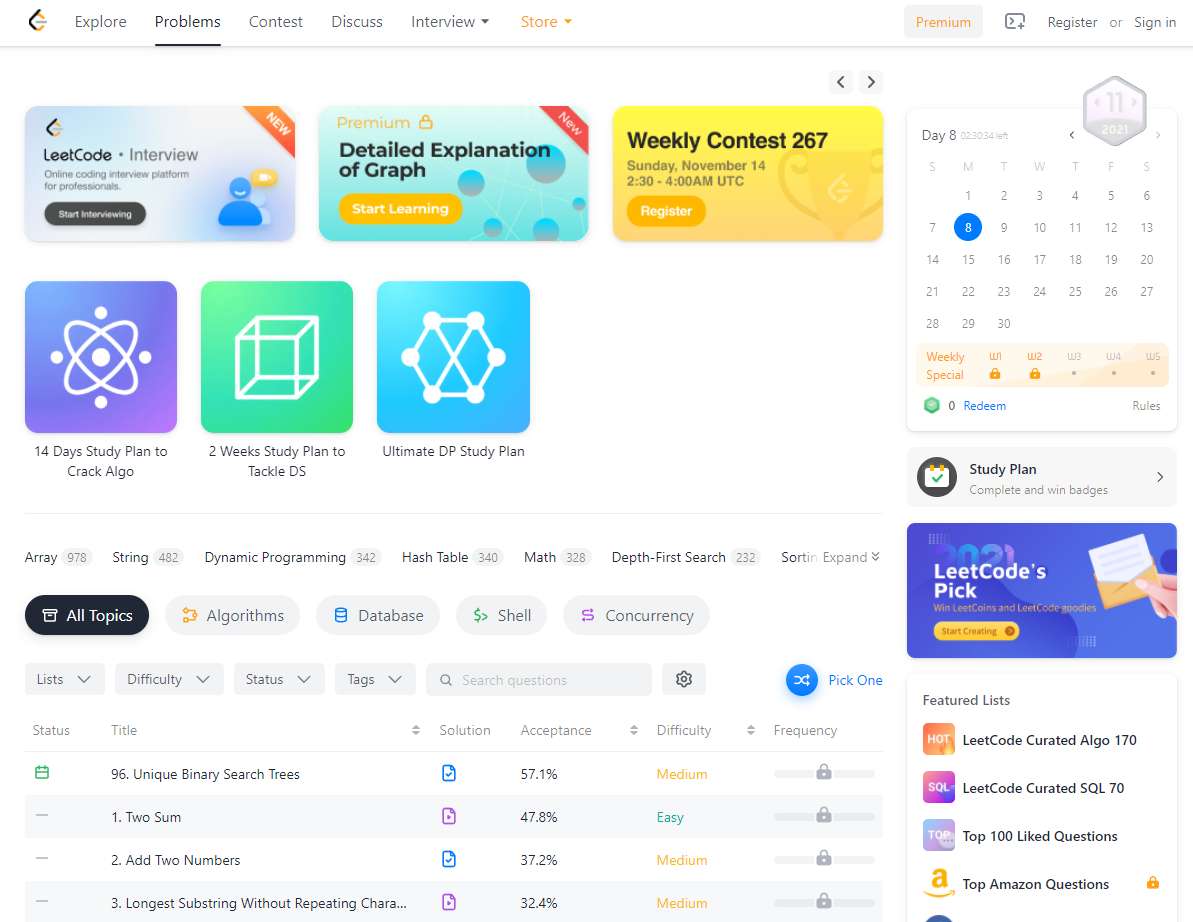
\includegraphics[width=\textwidth]{slike/leetcode.PNG} %veličina u odnosu na širinu linije
			\caption{\url{https://leetcode.com/problemset/all/}}
			\label{fig:leetcode} %label mora biti drugaciji za svaku sliku
		\end{figure}
		
		
		
		
		
	
		
	
		
	